\documentclass[12pt]{article}

\setlength{\topmargin}{-.75in} \addtolength{\textheight}{2.00in}
\setlength{\oddsidemargin}{.00in} \addtolength{\textwidth}{.75in}

\usepackage{amsmath,color,graphicx,array,multirow,rotating, enumerate}
\usepackage{type1cm}
\usepackage{eso-pic}
\usepackage[hmargin=2cm,vmargin=1.3cm]{geometry}
\usepackage{mathabx}
\usepackage[rflt]{/Users/jgates/desktop/latex/floatflt}
\usepackage[table]{xcolor}
\nofiles

\def\Tab#1{\tabular[t]{>{\rule[-1ex]{0pt}{3ex}}c}#1\endtabular}
\newcolumntype{C}{@{}c@{}}

\pagestyle{empty}
\newcounter{ProbNum}
\setlength{\parindent}{0in}

% Watermark: graph paper
\newcommand\BackgroundPic{
\put(0,0){
\parbox[b][\paperheight]{\paperwidth}{%
\vfill
\centering

\includegraphics[width=\paperwidth,height=\paperheight,keepaspectratio]{/Users/jgates/desktop/latex/pics/plain.pdf}%
\vfill
}}}

%Diagram box command [v space][content]
\newcommand{\diagrambox}[2][40 mm]{
\framebox{\parbox{175 mm}{#2 \hfill \\ \vspace{#1}}}

\bigskip
}

% MakeList: [example number] [content]
\newcommand{\MakeList}[2]{
\begin{enumerate}[#1] \itemsep1pt \parskip0pt \parsep0pt  

#2
\end{enumerate}
}

\begin{document}



% Name section
\noindent {\sc {\bf {\Large Reyes, Sofi }} \hfill
C15-Phases}

\noindent {\sc Physics 1/2 }\hfill {\large 4/09}
\bigskip

% Questions section
% Number 20
% UFPM CAPM Friction KFriction 
% Box sliding down frictionless incline: a, motion

% Watermark
\AddToShipoutPicture*{\BackgroundPic}

\addtocounter {ProbNum} {1}

\begin{floatingfigure}[r]{.25\textwidth}
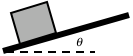
\includegraphics{/Users/jgates/desktop/latex/pics/incline1.png}
\end{floatingfigure} 

{\bf \Large{\arabic{ProbNum}}} A box of mass ${m}$ slides with an initial velocity of ${3~\tfrac{m}{s}}$ down a ramp which is inclined ${20^\circ}$ from the horizontal.  The coefficient of kinetic friction between the ramp and box is .45.

\bigskip

\indent  a. Determine the direction and magnitude of the acceleration of the box as it slides down the incline. 

\vfill

b. Discuss the subsequent motion of the box (qualitatively - no numbers are necessary).

\vspace{25mm}

\newpage
% Number 50
% UFPM GM UCM
% Simple circular orbit - geosynch

% Watermark
\AddToShipoutPicture*{\BackgroundPic}

\addtocounter {ProbNum} {1}

{\bf \Large{\arabic{ProbNum}}} ${\left ( G = 6.67 \times 10^{-11}~\tfrac{Nm^2}{kg^2} \right )}$ A satellite is said to be in \emph{geosynchronous orbit} if it always stays above the same spot on the body that it is orbiting.  It accomplishes this by having the same orbital period as the rotational period of the body that is it orbiting. (How long is that for the Earth?)

\bigskip

a. Determine how far from the surface of the Earth a satellite must be placed in order to be in a geosynchronous orbit. ${\left ( R_{\Earth} = 6,370~km; M_{\Earth}=5.97 \times 10^{24}~kg \right )}$

\vfill

b. The space shuttle orbits the Earth with a period of around 90 minutes.  Is it closer to the Earth or further from the Earth than geosynchronous satellites?  Be convincing!

\vspace{25mm}
 
\newpage


% Standards section
\centering
{\footnotesize \begin{tabular}{| p{.35 cm} | p{1.7 cm} | p{14.3 cm} | }
\hline
\multirow{8}{*}{\begin{sideways}\parbox{4mm}{{\large{\bf Friction}}}\end{sideways}}  &Core Skills 		& Draw an IF chart describing momentum before and after an interaction  \\ \cline{3-3}
& 					& Treat momentum as a vector, correctly and consistently  \\ \cline{2-3}					
& \multirow{2}{*}{\parbox{1.7cm}{Proficiency Indicators}}	& Identify situations in which momentum is conserved \\ \cline{3-3}
&					& Write an accurate conservation equation describing the system \\ \cline{3-3}
& 					& Distinguish among inelastic, completely inelastic, and elastic collisions \\ \cline{3-3}
& 					& Determine the change in kinetic energy due to a collision \\ \cline{3-3}
&					& Analyze elastic collisions using the speeds of approach and retreat \\ \cline{2-3}
& Advanced Indicators	& Analyze collisions using the center-of-mass reference frame \\ \hline
\end{tabular} }
\vspace{2 mm}


\centering
{\footnotesize \begin{tabular}{| p{.35 cm} | p{1.7 cm} | p{14.3 cm} | }
\hline
\multirow{8}{*}{\begin{sideways}\parbox{4mm}{{\large{\bf CAPM}}}\end{sideways}}  &Core Skills 		& Draw an IF chart describing momentum before and after an interaction  \\ \cline{3-3}
& 					& Treat momentum as a vector, correctly and consistently  \\ \cline{2-3}					
& \multirow{2}{*}{\parbox{1.7cm}{Proficiency Indicators}}	& Identify situations in which momentum is conserved \\ \cline{3-3}
&					& Write an accurate conservation equation describing the system \\ \cline{3-3}
& 					& Distinguish among inelastic, completely inelastic, and elastic collisions \\ \cline{3-3}
& 					& Determine the change in kinetic energy due to a collision \\ \cline{3-3}
&					& Analyze elastic collisions using the speeds of approach and retreat \\ \cline{2-3}
& Advanced Indicators	& Analyze collisions using the center-of-mass reference frame \\ \hline
\end{tabular} }
\vspace{2 mm}



{\footnotesize \begin{tabular}{| p{.15 cm}  p{.15 cm} | p{1.7 cm} | p{13 cm} | }
\hline
\multirow{8}{*}
{\rotatebox[origin=c]{90}{\parbox{32 mm}{{\large{\bf UFPM }}}}}  
&\multirow{8}{*}
{\rotatebox[origin=c]{90}{{\parbox{50 mm}{\scriptsize \centering Unbalanced Force Particle Model}}}} &Core Skills 	& Recognize when the forces on an object or system are not balanced from observation, graphs, equations, or descriptions of the motion  \\ \cline{4-4}
& & 					& Identify the presence and directions of normal, tension, and weight forces  \\ \cline{4-4}
& & 					& Draw a force diagram (FBD) accurately showing directions and types of forces acting on an object or system  \\ \cline{4-4}	
& & 					& Write net force equations describing an object or system; they should indicate that the forces are not balanced in the appropriate dimension(s)  \\ \cline{3-4}											
& & \multirow{2}{*}{\parbox{1.7cm}{Proficiency Indicators}}	& Draw FBD correctly indicating that forces are not balanced; recognize same \\ \cline{4-4}
& &					& Choose and consistently apply workable direction(s) of positive \\ \cline{4-4}
& &					& Correctly apply Newton's 3rd law \\ \cline{4-4}
& & 					& Choose appropriate axes for force analysis \\ \cline{4-4}
& & 					& Solve problems using net force equations and/or FBD \\ \cline{3-4} 
 \hline
\end{tabular} }
\vspace{2 mm}

\centering
{\footnotesize \begin{tabular}{| p{.35 cm} | p{1.7 cm} | p{14.3 cm} | }
\hline
\multirow{8}{*}{\begin{sideways}\parbox{4mm}{{\large{\bf UCM}}}\end{sideways}}  &Core Skills 		& Draw an IF chart describing momentum before and after an interaction  \\ \cline{3-3}
& 					& Treat momentum as a vector, correctly and consistently  \\ \cline{2-3}					
& \multirow{2}{*}{\parbox{1.7cm}{Proficiency Indicators}}	& Identify situations in which momentum is conserved \\ \cline{3-3}
&					& Write an accurate conservation equation describing the system \\ \cline{3-3}
& 					& Distinguish among inelastic, completely inelastic, and elastic collisions \\ \cline{3-3}
& 					& Determine the change in kinetic energy due to a collision \\ \cline{3-3}
&					& Analyze elastic collisions using the speeds of approach and retreat \\ \cline{2-3}
& Advanced Indicators	& Analyze collisions using the center-of-mass reference frame \\ \hline
\end{tabular} }
\vspace{2 mm}


\centering
{\footnotesize \begin{tabular}{| p{.35 cm} | p{1.7 cm} | p{14.3 cm} | }
\hline
\multirow{8}{*}{\begin{sideways}\parbox{4mm}{{\large{\bf GM}}}\end{sideways}}  &Core Skills 		& Draw an IF chart describing momentum before and after an interaction  \\ \cline{3-3}
& 					& Treat momentum as a vector, correctly and consistently  \\ \cline{2-3}					
& \multirow{2}{*}{\parbox{1.7cm}{Proficiency Indicators}}	& Identify situations in which momentum is conserved \\ \cline{3-3}
&					& Write an accurate conservation equation describing the system \\ \cline{3-3}
& 					& Distinguish among inelastic, completely inelastic, and elastic collisions \\ \cline{3-3}
& 					& Determine the change in kinetic energy due to a collision \\ \cline{3-3}
&					& Analyze elastic collisions using the speeds of approach and retreat \\ \cline{2-3}
& Advanced Indicators	& Analyze collisions using the center-of-mass reference frame \\ \hline
\end{tabular} }
\vspace{2 mm}


\end{document}